\documentclass[t,compress]{beamer}
%\documentclass[t,compress,handout]{beamer}
\usepackage{Rcolour}
\graphicspath{{../../graphics/}}

 
\usepackage{amsmath,amsfonts,amssymb,psfrag,epsfig,subfigure,ncsg3}
\usepackage{comment,color,xspace,pdfpages,wasysym}
\usepackage[normalem]{ulem} 
\usepackage{listings,booktabs} 
\usepackage{termcal}
\usepackage[english]{babel}

\usetheme{Madrid}
\pagestyle{empty}
%
\setcounter{section}{0}




%\RequirePackage[osf,sc]{mathpazo}{}
\RequirePackage[scaled=0.90]{helvet}{}
\RequirePackage[scaled=0.85]{beramono}{}
\RequirePackage[T1]{fontenc}
\RequirePackage{textcomp}
\graphicspath{{graphics/}}
%%%%%%%%%%%%%%%%%%%%%%%%%%%%%%%%%%%%%%%%%%%%%%%%%%%%%%%%%%%%%%%%%%%%%
%%%%%%%%%%%%%%%%%%%%%%%%%%%%%%%%%%%%%%%%%%%%%%%%%%%%%%%%%%%%%%%%%%%%%
%%%%%%%%%%%%%%%%%%%%%%%%%%%%%%%%%%%%%%%%%%%%%%%%%%%%%%%%%%%%%%%%%%%%%
\title[Approximate accelerated stochastic simulation of chemically reacting systems]{Approximate accelerated stochastic simulation of chemically reacting systems}

\author[]{Colin Gillespie}

\date{\today}
%%%%%%%%%%%%%%%%%%%%%%%%%%%%%%%%%%%%%%%%%%%%%%%%%%%%%%%%%%%%%%%%%%%%%
%%%%%%%%%%%%%%%%%%%%%%%%%%%%%%%%%%%%%%%%%%%%%%%%%%%%%%%%%%%%%%%%%%%%%
%%%%%%%%%%%%%%%%%%%%%%%%%%%%%%%%%%%%%%%%%%%%%%%%%%%%%%%%%%%%%%%%%%%%%
\begin{document}
\maketitle

\begin{frame}
\frametitle{Overview}
\begin{itemize}
\item Stochastic kinetic models
\item Issues with the Direct method
\item $\tau$-leap method (Gillespie, 2001)
\begin{itemize}
\item Leap conditions
\item Mid-point estimation
\end{itemize}
\item Examples
\end{itemize}
{\small
Source code (R and \LaTeX\ of these slides):\\
\alert{\url{https://github.com/csgillespie/talks/}}}

\end{frame}


\begin{frame}
\frametitle{Stochastic kinetic models}

\noindent A biochemical network is represented as a set of pseudo-biochemical reactions:
\begin{block}{$u$ species \& $v$ reactions}
\[
R_i:\quad p_{11}\mathcal{X}_1+p_{12}\mathcal{X}_2+\cdots+p_{1u}\mathcal{X}_u 
\xrightarrow{c_i}
q_{11}\mathcal{X}_1+q_{12}\mathcal{X}_2+\cdots+q_{1u}\mathcal{X}_u
\]
Stochastic rate constant $c_i$.
\end{block}
Hazard/instantaneous rate: $h_i(X_t, c_i)$ where $X_t = (X_{1,t}, \ldots, X_{u,t})′$ is
the current state of the system.

Under mass-action stochastic kinetics, the hazard function is proportional to a
product of binomial coefficients, with
\[
h_i(X_t,c_i) = c_i\prod_{j=1}^u \binom{X_{j,t}}{p_{ij}}.
\]

\end{frame}

\begin{frame}
\frametitle{Stochastic kinetic model}
\begin{itemize}
\item Describe the SKM by a Markov jump process (MJP)
\item The effect of reaction $R_k$ is to change the value of each species $X_i$ by
$q_{ji} - p_{ji}$
\item The stoichiometry matrix $S$ has elements $s_{ij} = q_{ji} - p_{ji}$
\item It can be shown that the time to the next reaction is
\[
t \sim Exp(h_0 (X_t , c))
\quad\text{where}\quad
h_0(X_t , c) =\sum_{i=1}^v h_i(X_i, c_i)
\]
and the reaction is of type $i$ with probability $h_i(X_t, c_i)/h_0(X_t , c)$
\item The process is easily simulated using the Direct method (Gillespie algorithm)
\end{itemize}
\end{frame}


\begin{frame}
\frametitle{Example: Lotka-Volterra system}
\begin{columns}[c]
\column{0.58\textwidth}
\begin{itemize}
\item $R_1$: Prey reproduction
\[
 \mathcal{X}_{1}\xrightarrow{\phantom{a}c_{1}\phantom{a}}  2\mathcal{X}_{1}
\]
\item $R_2$: Prey death, predator reproduction
\[
  \mathcal{X}_{1}+\mathcal{X}_{2}\xrightarrow{\phantom{a}c_{2}\phantom{a}}
  2\mathcal{X}_{2} 
\]
\item $R_3$: Predator death
\[
   \mathcal{X}_{2}\xrightarrow{\phantom{a}c_{3}\phantom{a}}  \emptyset 
\]
\end{itemize}


\column{0.4\textwidth}
\begin{figure}
\centering
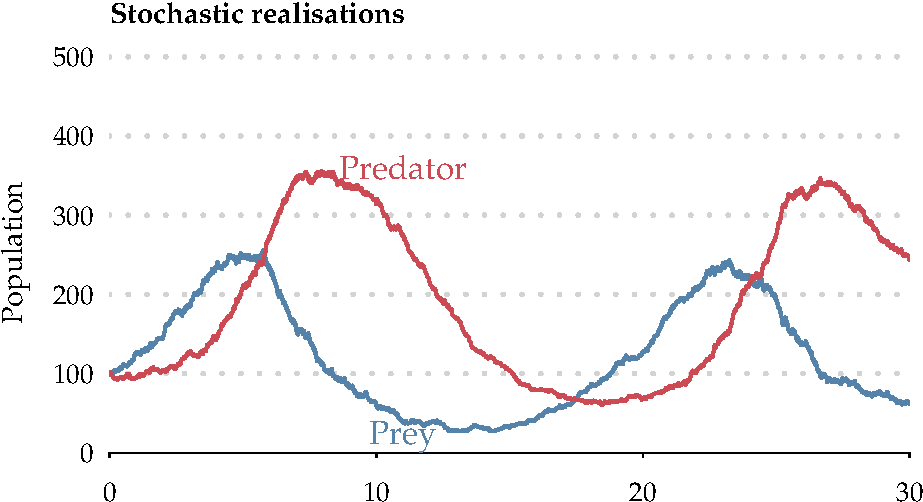
\includegraphics[width=\textwidth]{figure1a-crop}\\
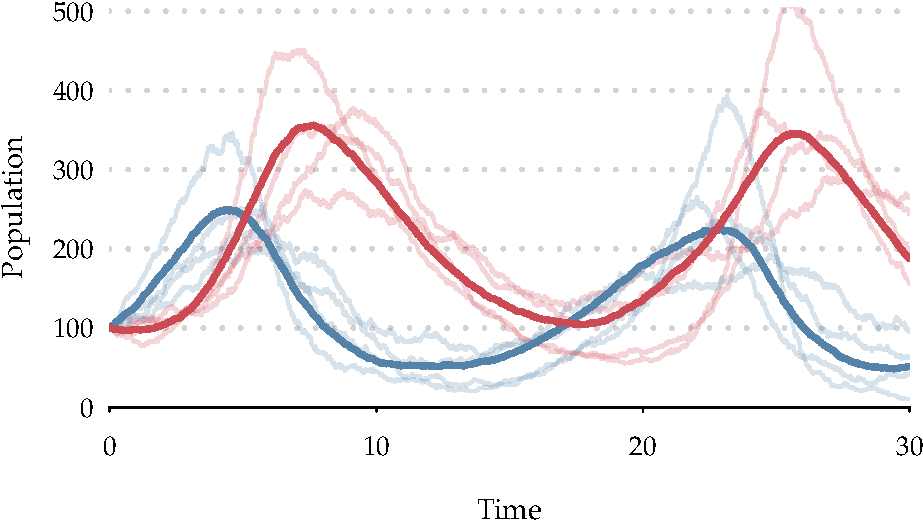
\includegraphics[width=\textwidth]{figure1b-crop}
\end{figure}
$\mathbf{X(0)} = (100, 100)$\\  $\mathbf{c} = (0.5, 0.0025, 0.3)$
\end{columns}
\end{frame}

\begin{frame}
\frametitle{The direct method}

\begin{enumerate}
\item \textbf{Initialisation:} initial conditions, reactions constants, and random number generators
\item \textbf{\alert<2>{Propensities update:}} Update each of the $v$ hazard functions, $h_i(x)$
\item \textbf{Propensities total:} Calculate the total hazard $h_0 = \sum_{i=1}^v h_i(x)$
\item \textbf{\alert<3>{Reaction time:}} $\tau = -ln[U(0,1)]/h_0$ and $t = t+ \tau$
\item \textbf{\alert<4>{Reaction selection:}} A reaction is chosen proportional to it's
  hazard
\item \textbf{Reaction execution:} Update species
\item \textbf{Iteration:} If the simulation time is exceeded stop, otherwise go back to step 2
\end{enumerate}
\alert<2->{Typically there are a large number of iterates}
\end{frame}


\begin{frame}
  \frametitle{Approximations} 

Relax some assumptions (e.g. discreteness  and stochasticity) in order to make simulation faster and more scalable
\begin{itemize}
\item Diffusion approximation / chemical Langevin equation (CLE)
\item Linear noise approximation (LNA) / moment closure (2MA)
\item ODE
\item Hybrid discrete-continuous models
\end{itemize}
\end{frame}

\begin{frame}
\frametitle{Poisson leap}
\begin{itemize}
\item If all reactions are zeroth-order, then the model is a homogeneous Poisson process
\item Hence the number of reactions in $(t_0, t_1)$ follows a Poisson distribution
\item For a more general model, if we consider a \textit{small} time interval,
  $(t, t+ \Delta t)$, then:
\begin{itemize}
\item the hazard rates should be approximately constant
\item the number of reactions (of a given type) can be sampled from a Poisson
  distribution
\end{itemize}
\item A balance between speed and accuracy
\end{itemize}
\end{frame}

\begin{frame}
\frametitle{Poisson leap method}
\begin{enumerate}
\item Set $t=0$. Initialise the rate constants and the initial molecule numbers $x$
\item Calculate $h_i(x,c_i)$, for $i=1,\ldots,v$, and simulate the
$v$-dimensional reaction vector $r$, with $i^{\text{{\tiny th}}}$ entry a
$Po(h_i(x,c_i)\Delta t)$ random quantity
\item Update the state according 
\item Update $t:=t+\Delta t$
\item Output $t$ and $x$. If $t<T_{max}$ return to step 2
\end{enumerate}
\pause
\begin{center}
{\Large {\color{red}How do you chose $\Delta t$?}}
\end{center}
\end{frame}

\begin{frame}
\frametitle{Example: Lotka-Volterra}

\begin{columns}[t]
\column{0.45\textwidth}
\begin{itemize}
\item Suppose we are interested in parameter inference
\item A possible prior could be independent Uniform priors over $U(-8, 8)$ for
  each $\log(c_i)$
\item Three samples from this prior yield very different realisations
\begin{itemize}
\item Probability of extinction by time $t=30$, is around 0.86
\end{itemize}
\item Each simulation would require a very different $\Delta t$
\end{itemize}
\column{0.55\textwidth}
\vspace{-1cm}
\begin{figure}
\centering
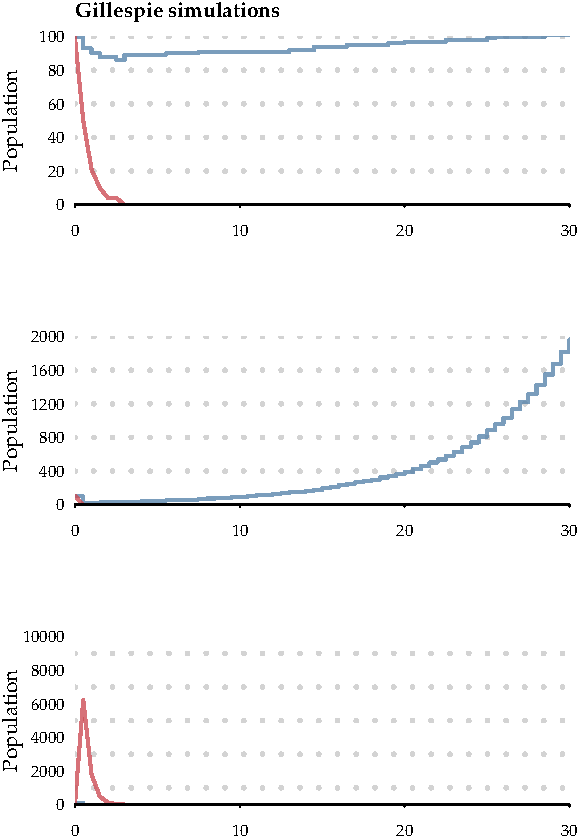
\includegraphics[width=0.8\textwidth]{figure2-crop}
\end{figure}
\vfill
\end{columns}
\end{frame}


\begin{frame}
\frametitle{Basic $\tau$-leap method}
\begin{itemize}
\item Suppose a temporal leap $\tau$ will result in a state change $\mathbf{\lambda}$
\item Choose a value of $\tau$ that satisfies the \textit{leap condition}. For
  each reaction, $R_j$, we want
\[
\vert h_j(\mathbf{x} + \mathbf{\lambda} )- h_j(\mathbf{x}) \vert 
\]
to be \textit{small}
\item Sample $k_j \sim P(h_j(\mathbf{x})\tau)$
\item Compute $\mathbf{\lambda}$
\item Set $t:= t + \tau$ and $\mathbf{x}:= \mathbf{x} + \mathbf{\lambda}$
\end{itemize}
\end{frame}

\begin{frame}
\frametitle{Choosing $\tau$}
\begin{itemize}
\item If the reactions don't depend on $\mathbf{x}$, the leap condition will be
  satisfied exactly for any $\tau$ (and so exact)
\item If population numbers are large, then it would take a large number of
  reactions to ``noticeably'' change the hazard functions
\item If satisfying the leap condition requires a very small value $\tau <<
  1/h_0(\mathbf{x})$, then we may as well use the exact SSA
\end{itemize}
\end{frame}


\begin{frame}
\frametitle{A procedure for selecting $\tau$ (Gillespie 2001)}
\begin{itemize}
\item The expected net change in $(t, t+\tau)$ will be:
\[
\bar{\mathbf{\lambda}} = \sum_{j=1}^v [h_j(\mathbf{x}) \tau] \mathbf{s}_j = \tau
\mathbf{\xi(x)}
\]
\item So we require that the \textit{expected} changes in the propensity functions in time
  $\tau$, are bounded by some fraction of all propensity functions, i.e.
\[
\vert  h_j(\mathbf{x} + \mathbf{\lambda} )- h_j(\mathbf{x}) \vert < \epsilon h_0
(\mathbf{x}) \quad \text{for } j=1, \ldots, v.
\]
\item Estimate the difference using a Taylor expansion:
\[
h_j(\mathbf{x} + \mathbf{\lambda} )- h_j(\mathbf{x}) \simeq \sum_{i=1}^u \tau
\xi_i(\mathbf{x}) \frac{\partial}{\partial x_i} h_j(\mathbf{x})
\]
\item Defining
\[
b_{ji}(\mathbf{x}) \equiv \frac{\partial h_j(\mathbf{x})}{\partial x_i} \quad (j=1,
 \ldots, v; i=1, \ldots, u)
\]
\end{itemize}
\end{frame}
\begin{frame}
\frametitle{A procedure for selecting $\tau$}
\begin{itemize}
\item The requirement becomes
 \[
 \tau \left\vert \sum_{i=1}^u \xi_i(\mathbf{x}) b_{ji}(\mathbf{x}) \right \vert
 \le \epsilon h_0(\mathbf{x}) \quad (j=1, \ldots, v)
 \]
\item The largest value of $\tau$ consistent with this condition (and hence
  optimal) is
\[
\tau = \min_{j\in [1, v]} \left\{  \frac{\epsilon h_0(\mathbf{x})}{\left\vert
      \sum_{i=1}^u \xi_i(\mathbf{x}) b_{ji}(\mathbf{x}) \right \vert} \right\}
\]
Typical values of $\epsilon$ are around 0.05
\end{itemize}
\end{frame}

\begin{frame}
\frametitle{Example: Lotka-Volterra}

\begin{figure}
\centering 
\only<1>{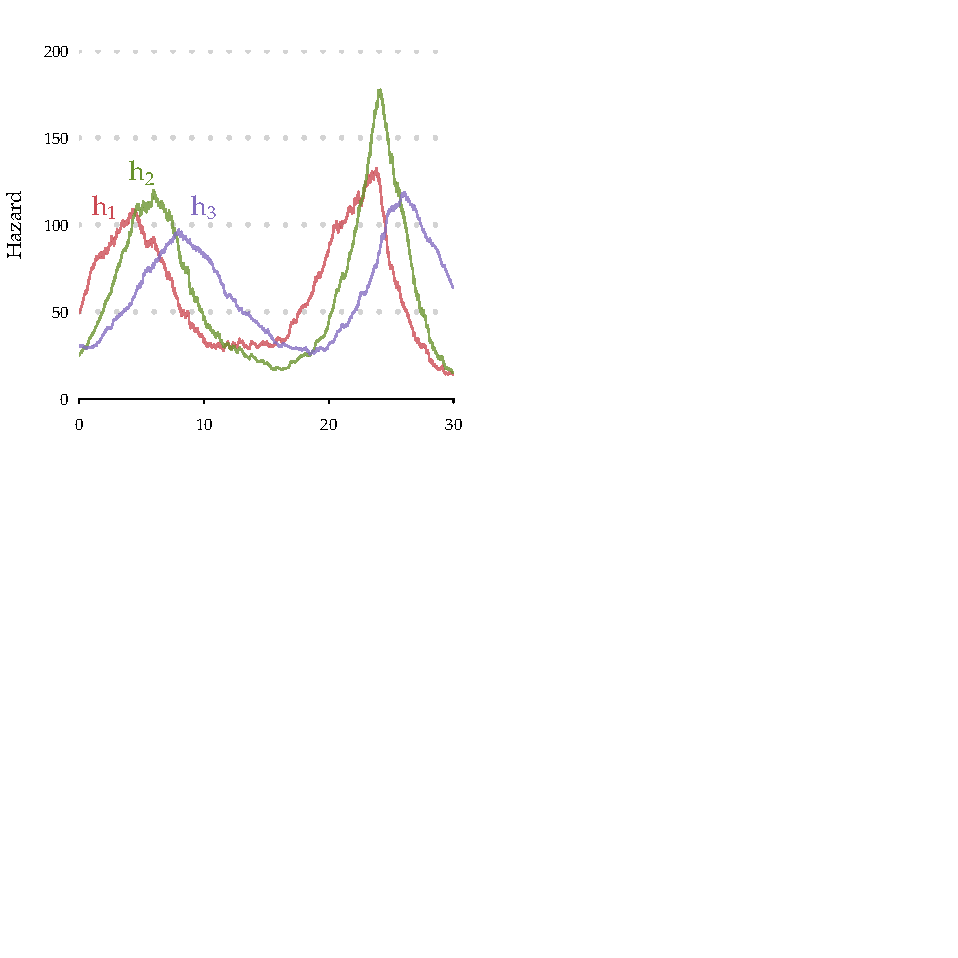
\includegraphics[width=8cm]{figure4a}}%
\only<2>{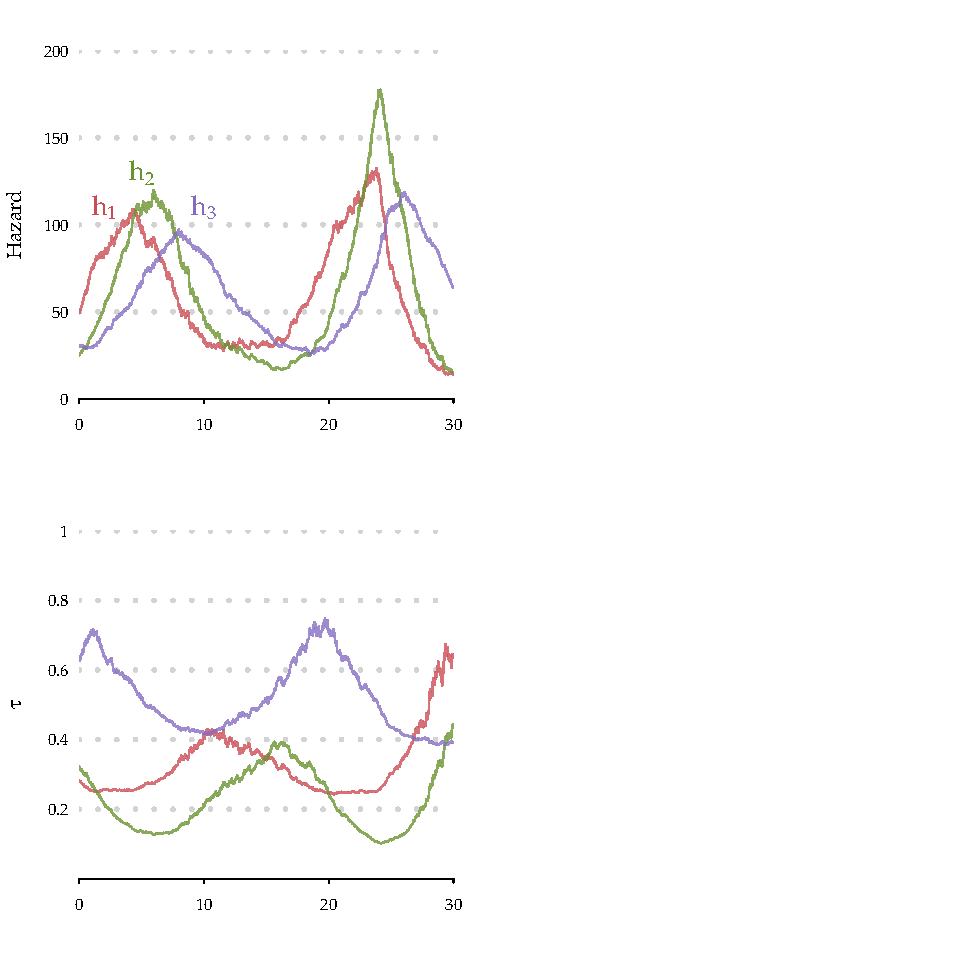
\includegraphics[width=8cm]{figure4b}}%
\only<3>{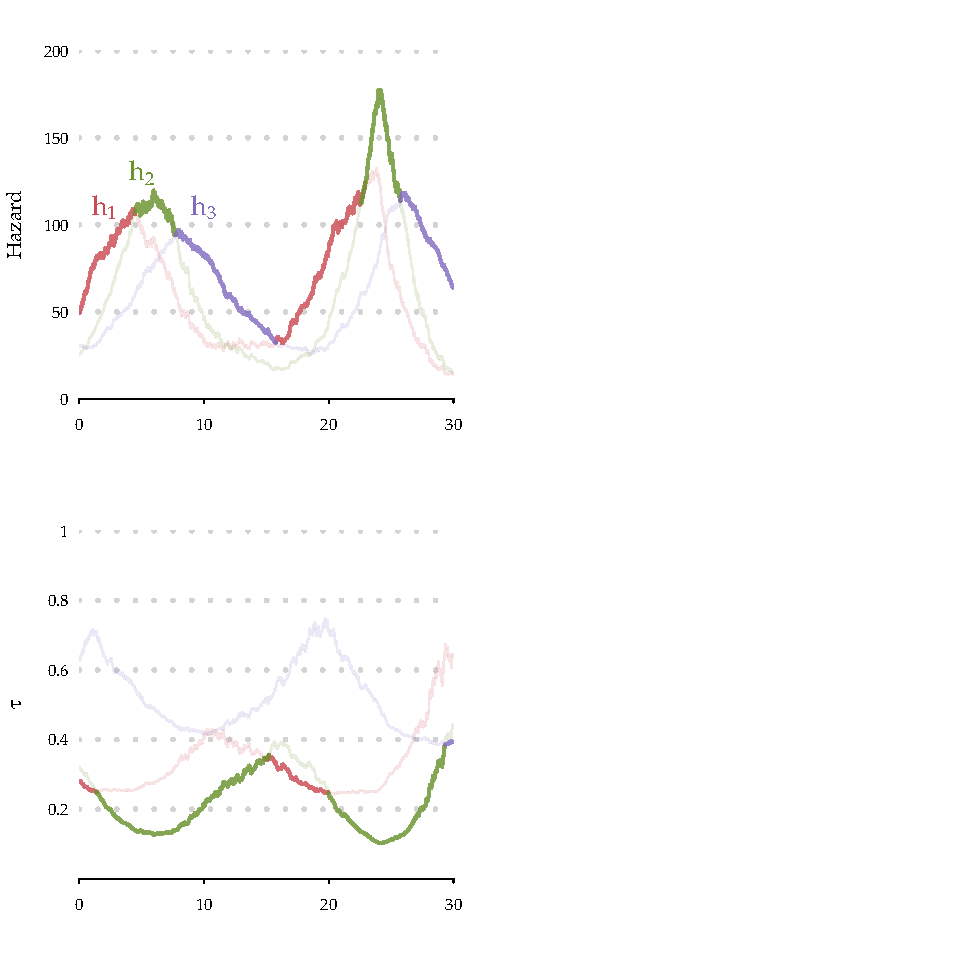
\includegraphics[width=8cm]{figure4c}}%
\only<4->{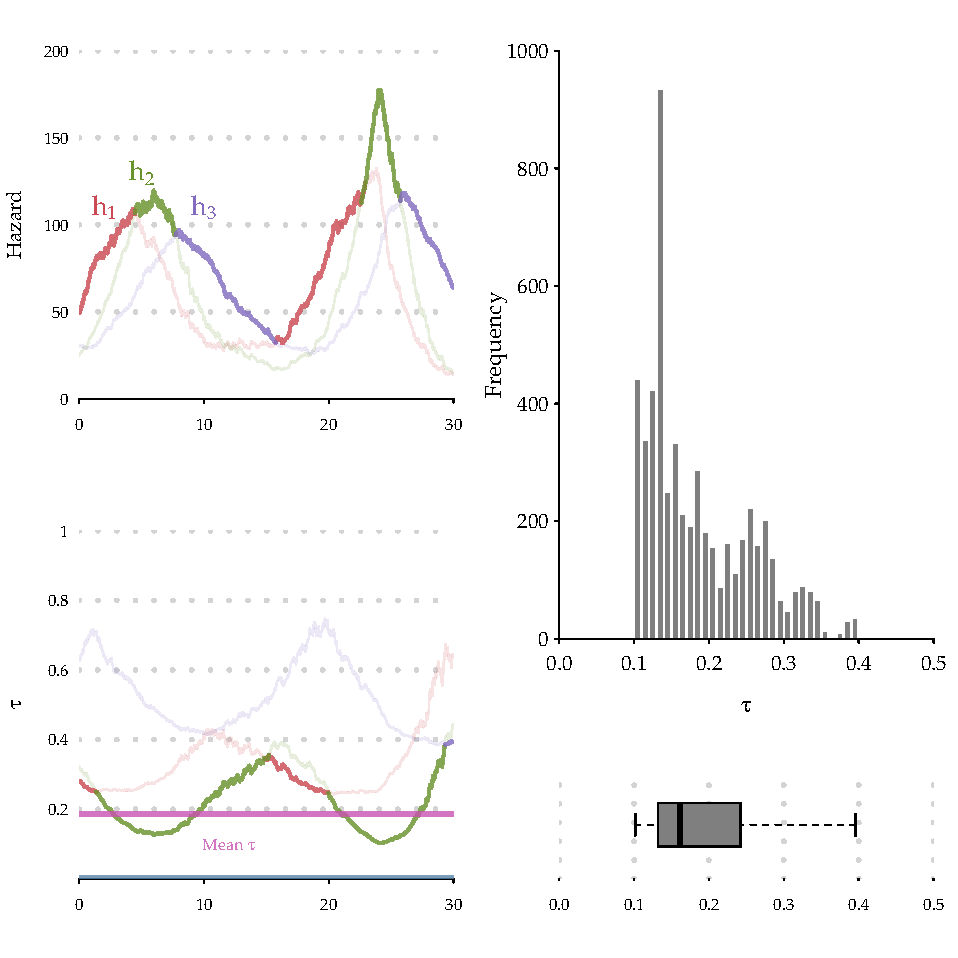
\includegraphics[width=8cm]{figure4d}}%
\end{figure}
\end{frame}




\begin{frame}
\frametitle{The estimated-midpoint technique}

\begin{itemize}
\item The leap condition requires that the hazards functions do not
  ``appreciably'' change in the course of a leap
\item But we want to take large leaps, so we will inevitably get computational errors
\item This is similar to solving the ODE
\[
\frac{dX(t)}{dt} = f(X)
\] 
using an Euler scheme
\item A standard technique is to use a \textit{second-order Runge-Kutta} or \textit{modified Euler} method
\[
X(t + \Delta t) = X(t) + f[X(t) + 0.5 f(X(t)) \Delta t] \Delta t
\]
i.e. we use an Euler method to estimate the midpoint during $[t, t+\Delta t]$, then calculate the increment in $X$ by evaluating the slope function $f$ at that
estimated midpoint
\end{itemize}

\end{frame}



\begin{frame}
\frametitle{Example: Death model}

\begin{itemize}
\item The death model contains a single reaction
\[
\mathcal{X}\xrightarrow{\phantom{a}\mu \phantom{a}}  \emptyset
\]
and has hazard function $h_1(x, \mu) = \mu x$ and state change vector $s=-1$.
\item The solution to the CME is:
\[
\Pr(X=x; t) = \binom{x_0}{x} e^{-\mu \tau(x_0-x)} (1-e^{-\mu \tau })^x
\]
\end{itemize}
\end{frame}





\begin{frame}
  \frametitle{Death model} 
\vspace{-0.6cm}
\begin{figure}[t]
\centering
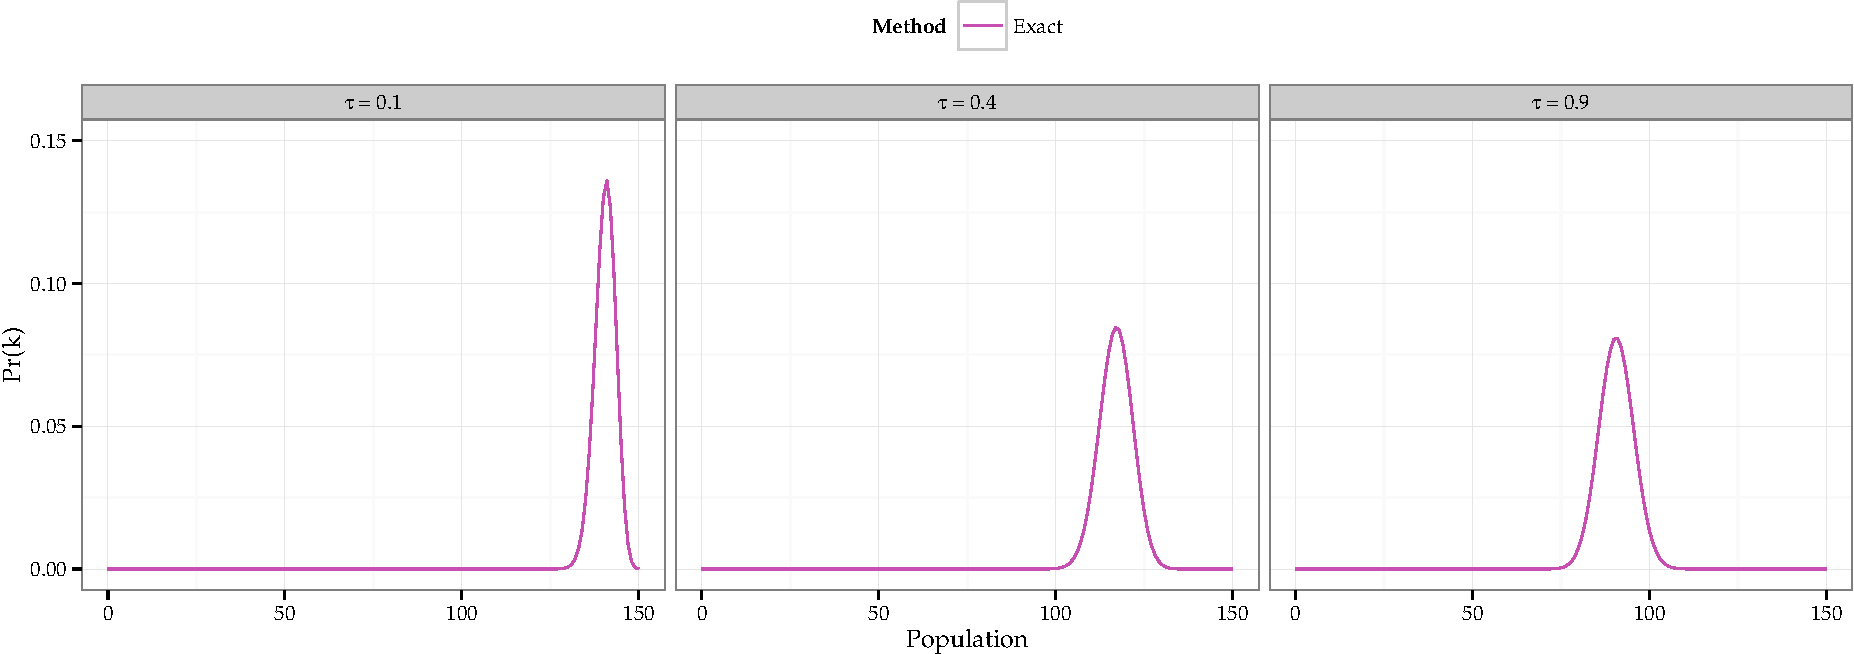
\includegraphics[width=\textwidth]{figure3a-crop}

\end{figure}
\[
\Pr(X=x; \tau) = \binom{x_0}{x} e^{-\mu \tau(x_0-x)} (1-e^{-\mu \tau })^x
\]
\end{frame}



\begin{frame}
  \frametitle{Death model: p-leap} 
\vspace{-0.6cm}
\begin{figure}[t]
\centering
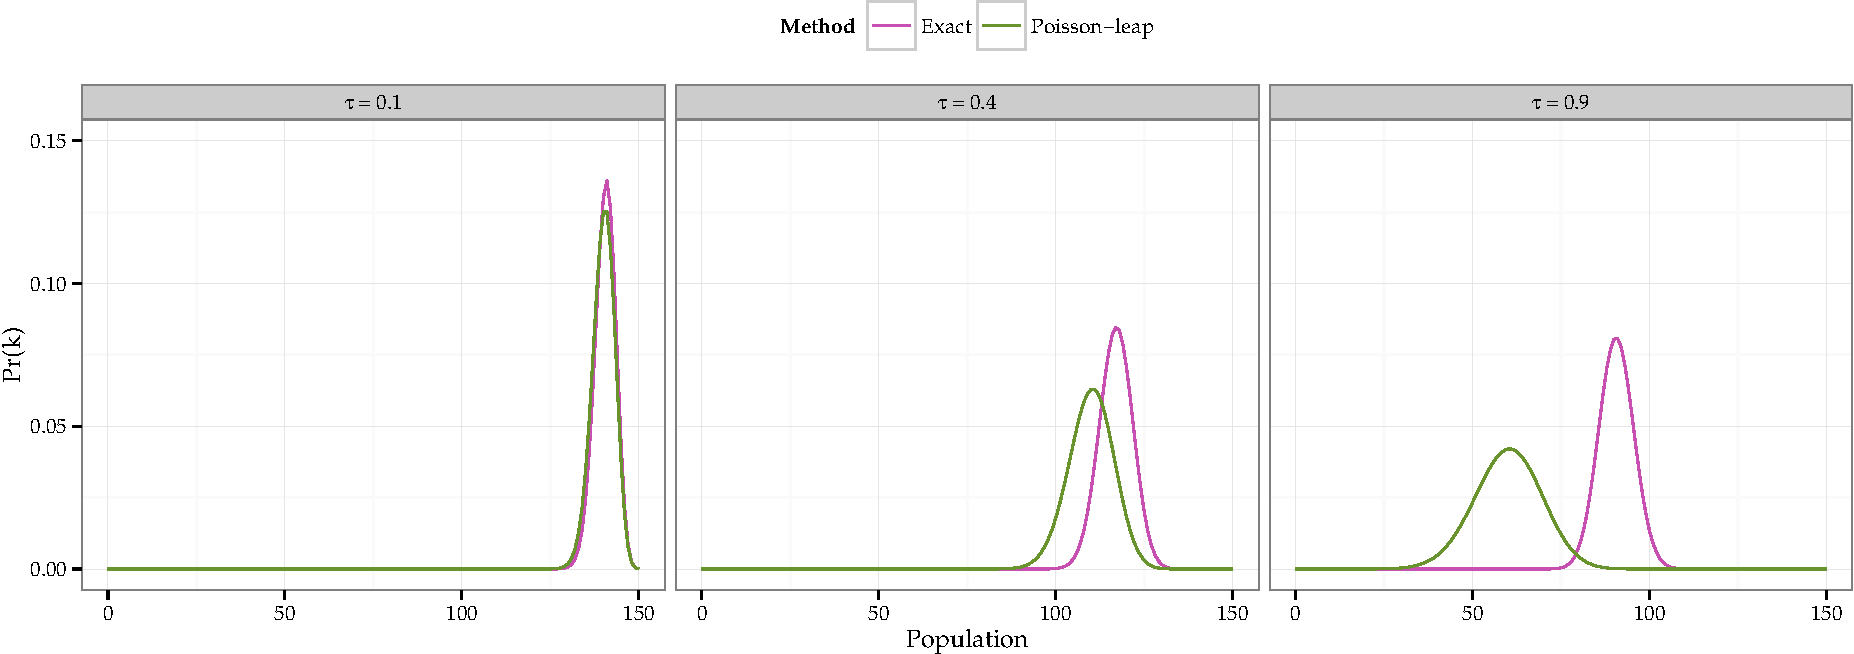
\includegraphics[width=\textwidth]{figure3b-crop}
\end{figure}
If we perform a single leap of length $\tau$, the number of executed reactions are
\[
P_p(k; \mu x_0, \tau) =\frac{e^{\mu x_0 \tau} (\mu x_0 \tau)^k}{k!} \quad
\text{for } k=0, \ldots
\]

\end{frame}



\begin{frame}
  \frametitle{Death model: $\tau$-leap + mid-point}
\vspace{-0.6cm}
\begin{figure}[t]
\centering 
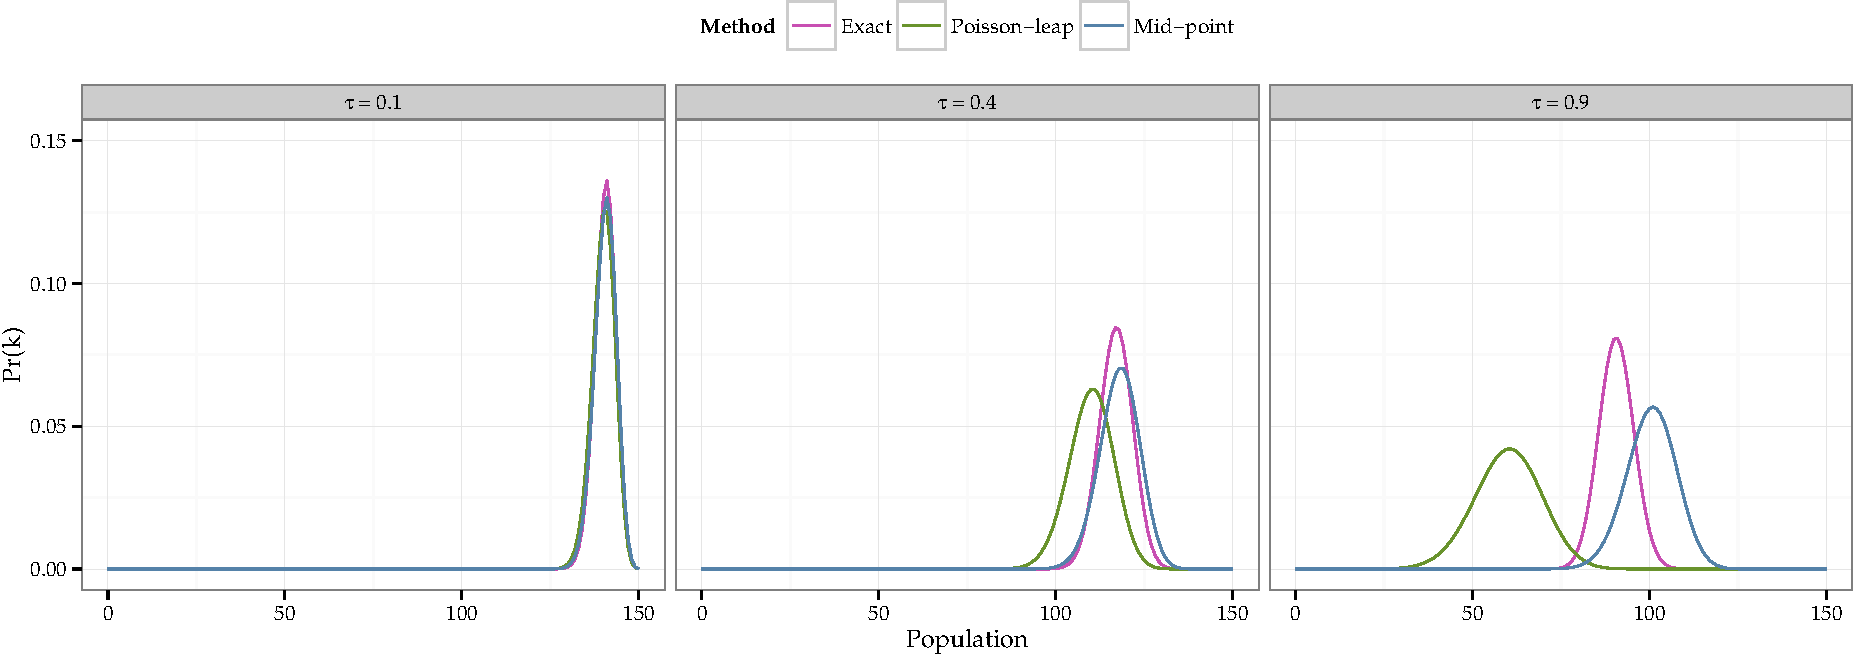
\includegraphics[width=\textwidth]{figure3c-crop}
\end{figure}
We estimate the mid-point to be:
\[ 
x' \equiv x_0 - \lfloor 0.5 \tau \mu x_0 \rfloor  
\]
so the number of reactions executed is
\[
P_p(k; \mu x_0, \tau) =\frac{e^{\mu x' \tau} (\mu x' \tau)^k}{k!} \quad
\text{for } k=0, \ldots
\]

\end{frame}

\begin{frame}
\frametitle{Example: Lotka-Volterra}

\begin{figure}
\centering
\only<1>{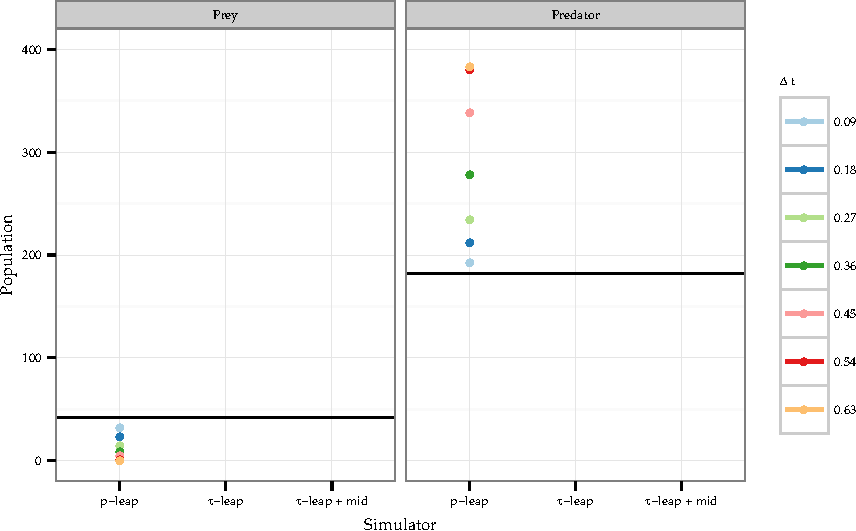
\includegraphics[]{figure5a-crop}}%
\only<2>{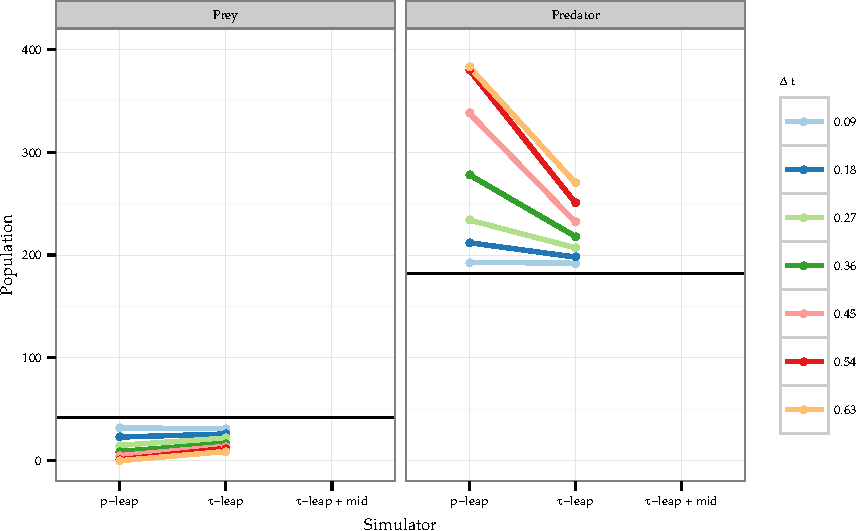
\includegraphics[]{figure5b-crop}}%
\only<3>{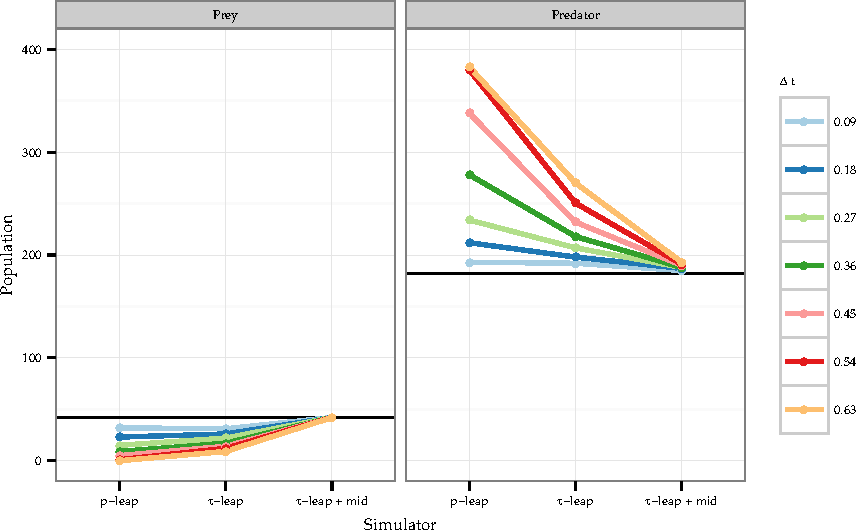
\includegraphics[]{figure5c-crop}}%
\end{figure}
\only<2->{For these parameter values and this model, we have the approximate
  relationship (obtained via simulation)
\[
\epsilon \simeq 0.556 \times \Delta t
\]
}
\end{frame}

\begin{frame}
\frametitle{Summary}
\begin{itemize}
\item Similar issues arise when solving SDEs with the Euler-Maruyama scheme
\begin{itemize}
\item In fact, if we substitute Poisson with Gaussian random numbers in the
  p-leap scheme, we get the Euler-Maruyama algorithm
\end{itemize}
\item Choosing a fixed $\Delta t$ for a wide range of parameter combinations
  doesn't make sense
\item Is it possible to these ideas when constructing bridges for SDEs?
\end{itemize}
\end{frame}

\begin{frame}
\frametitle{References}
{\small
\begin{itemize}
\item Gillespie DT. \textit{Exact stochastic simulation of coupled chemical
    reactions}. The Journal of Physical Chemistry, 1977, \textbf{81}: 2340 --
  2361. \alert{Direct method}
\item Gillespie, DT. \textit{Approximate accelerated stochastic simulation of
    chemically reacting systems.} The Journal of Chemical Physics, 2001, \textbf{115}: 1716. \alert{$\tau$-leap method}
\item Sandmann, W. \textit{Streamlined formulation of adaptive explicit-implicit
    tau-leaping with automatic tau selection.} Simulation Conference (WSC),
  Proceedings of the 2009 Winter. IEEE, 2009. \alert{Nice overview of the
    various $\tau$-leap flavours.}
\item Golightly, A \& Gillespie, CS. \href{https://github.com/csgillespie/In-silico-Systems-Biology}{\textit{Simulation of Stochastic Kinetic
    Models.}} In Silico Systems Biology. Humana Press, 2013, 169 -- 187.
  \alert{Overview of various SSA.}
\begin{itemize}
\item \url{https://github.com/csgillespie/In-silico-Systems-Biology}
\end{itemize}
\end{itemize}}
\end{frame}











\end{document}

%%% Local Variables: 
%%% mode: latex
%%% TeX-master: t
%%% End: 
